\documentclass[a4paper]{article}

%% Language and font encodings
\usepackage[english]{babel}
\usepackage[utf8x]{inputenc}
\usepackage[T1]{fontenc}

%% Sets page size and margins
\usepackage[a4paper,top=3cm,bottom=2cm,left=3cm,right=3cm,marginparwidth=1.75cm]{geometry}
\linespread{1.5}

%% Useful packages
\usepackage{amsmath}
\usepackage{graphicx}
\usepackage{subcaption}
\usepackage[colorinlistoftodos]{todonotes}
\usepackage[colorlinks=true, allcolors=blue]{hyperref}
\usepackage{booktabs}
\usepackage[flushleft]{threeparttable}


\graphicspath{ {./figs} }

\begin{document} %{{{

\title{Novelty, Familiarity, and the Success of Fanfictions among Readers} %{{{
\date{\today}
\maketitle %}}}

\begin{abstract}

\end{abstract}

What do people like? This puzzle is the main challenge for the creative industry, a multi-billion dollar sector that produces mumerous cultural products in the form of movies, TV shows and video games \cite{creativeindustries}. On one hand, novelty is central to creative works because people seek surprise when consuming such products \cite{hutter2011infinite}. But on the other hand, studies have shown that people also have a strong preference for familiarity. For example, often when people listen to music, they choose songs that they have already listened to \cite{thompson2014shazam}. Mere exposure to a certain stimuli can also increase people's preference for it \cite{zajonc1968attitudinal}, even when they are not aware of the exposure \cite{kunst1980affective}. The exposure effect is assumed to have an evolutionary basis, and has been verified by multiple experiments \cite{bornstein1989exposure}.

Leveraging the familiarity effect is therefore a core strategy to increase affinity. Repetition has long been utilized in cultural products including music and poetry \cite{huron2013psychological}. This trend can be also found in the contemporary popular culture, where many new releases are adaptations, remakes, and remixes \cite{manovich2007comes} of existing works. For example, the companies Marvel and DC have been making movies based on their popular comics, including many sequels, prequels and ``reboots'', many of which resulted in great successes. In an extreme case, the origin story of the Spider-man has been re-played in three movies since 2002 \cite{spiderman}. Market reception indicates that the audience welcome these products: out of the 10 highest-grossing movies of 2016, 8 are adaptions, sequels, remakes, or part of a movie universe \cite{2016film}. This number increased to 10 out of 10 in 2017 \cite{2017film}. 

To reconcile the apparent conflict between the preference for novelty and familiarity, the \emph{optimal differentiation hypothesis} \cite{thompson2017hit} has been widely adopted. It states that successful creative works are combinations of convention and innovation; the most popular ones are differentiated from previous works and their peers, but not \emph{too} different . In psychology, this is captured in the Wundt-Berlyne curve, which suggests that when exposed to novel stimuli, a perceiver's positive feelings first increase as novelty increases, until reaching a certain threshold; afterwards, further increasing novelty will lead to a decrease in positive feelings \cite{berlyne1970novelty}. Experiments have supported this hypothesis \cite{hargreaves1984effects} \cite{sluckin1980liking}, which has been used to study the success of a variety of cultural products. For example, Askin and Mauskapf found that songs with optimal differentiation are more likely to be on the top of the Billboad's Hot 100 charts \cite{askin2017makes}. Sreenivasan found a similar pattern for films \cite{sreenivasan2013quantitative}, and Mukherjee et al. found that in scientific publications, the highest-cited papers are grounded on mostly conventional, but partly novel combinations of previous works. 

However, most of these researches rely on external metrics to measure the success of creative works, such as the box office or  the Billboard chart. These are highly influenced by factors not directly relevant to a creative works' quality, such as advertisement and media coverage. In particular, the consumers' choices are largely shaped by the herding behavior. For example, it was found that being on the New York Times bestseller book list will cause an increase in sales \cite{sorensen2007bestseller}.  Even a ``faked'' popularity can be turned into real popularity as people are more likely to view creative works that they perceive to be popular \cite{salganik2008leading}. Therefore, such metrics may not accurately reflect the consumers' actual enjoyment of a cultural product. Moreover, as the features of cultural products vary significantly across genres, lengths, subjects, etc, it is hard to measure the novelty or conventionality of one piece against the others. 

Here, we instead study a special type of creative works that are directly created and consumed by fans --- fan works. Known formally as transformative works, they are creative works made by fans based on one or more original works (``canons'') \cite{wiki:transf_work}. For example, a story written by a contemporary fan about Sherlock Holmes in his retirement is considered a fan work. Although fan works can take multiple media types such as paiting, music and games, the most common type is creative writing: fanfictions. As a unique cultural phenomena, fanfictions have drawn attention from media studies and cultural studies \cite{thomas2011fanfiction}. However, most of the existing studies focus on the identity of fanfiction writers \cite{black2006language}, the practice of fanfiction writing \cite{LIT:LIT12061}, and the interaction between fans \cite{hills2015expertise}, and it is difficult to find studies that focus on fanfictions themselves as creative works.

Using fanfictions as subjects of study, we may avoid some of the complications mentioned above. The success of a fanfiction can be measured more directly with less influence from other media. In the service that we used to collect data, readers can give ``Kudos'' to each work, expressing that they enjoyed reading it, as well as leaving comments and bookmarks. As a subculture, fanfictions are usually not published as books nor featured in mainstream media, and there is no ``bestseller list'' for fanfictions, reducing the effect of the herding behavior. Additionally, most fanfictions are freely available in the Internet, so that the price is not a confounding factor. Moreover, because fans of a canon usually form communities known as fandoms \cite{wiki:fandom}, sharing the same context, fanfictions have less variation in subjects. Finally, because they are freely available as plain texts without the copyright issues, natural language processing methods can be readily applicable to operationalize novelty quantitatively.

With these advantages, we investigate how a fanfiction's novelty or familiarity influences its success. We use two methods to estimate the novelty of the fanfictions: one based on the word features, and one on the topic features, with respect to other fanfictions in the same fandom. A fanfiction is more novel if it has a large distance to other fanfictions published during the same time period in the feature space, and vice versa. Using statistical models, we found a negative relationship between a fanfiction's novelty and its success, consistent across both methods, suggesting that in disproval of the optimal differentiation hypothesis, fanfiction readers prefer familiarity and discourage novelty in general.


\section*{Results} 
We collect data from an online fanfiction archive, Archive of Our Own (AO3), which allows users to upload their fanfictions and categorizes them based on fandoms. Established in 2009, it has become one of the largest fan communities, with 1,313,000 users and 3,423,000 pieces of fanfictions by November 2017 \cite{ao3stats}.

AO3 classifies the fandoms based on medium: movies, TV shows, books, anime \& manga, and musicals, etc. We first list the top 5 fandoms in each category based on the number of fanfictions. Then we exclude the fandoms that are subsets of other large fandoms: for example, we keep \emph{Marvel} but exclude \emph{The Avengers}, since the fanfictions in \emph{The Avengers} are also in the \emph{Marvel} fandom. Fandoms that cover diverse topics such as \emph{k-pop} are also removed. We only kept the fictions written in English. Finally, to control for the effects of fiction length on the readers' preference and on our methods, we only analyze the fictions with 500 - 1500 words in each chapter, which is the range where most fictions lie (see Supp). This leaves us with 701,635 fanfictions in 24 fandoms.

\subsection*{Descriptive statistics}

Figure \ref{fig:fandom_size} shows the number of fanfictions in each of the 24 fandoms that we study. The fandoms with largest amounts of fictions are \emph{Marvel}, \emph{Supernatural}, and \emph{Harry Potter}. Figure \ref{fig:fic_time_dist}  shows the time distribution of the fanfictions published. As AO3 was established in December 2009, the fictions earlier than this time might be migrated from other platforms, and may not correctly reflect the status of the archive. We therefore only run our analysis using the fictions published in January 2010 and later. After the establishment, the site first experienced a slow growth until around 2012, when the number of fictions published begin to rise radically. 

\begin{figure}
    \centering
    \begin{subfigure}[b]{\textwidth}
        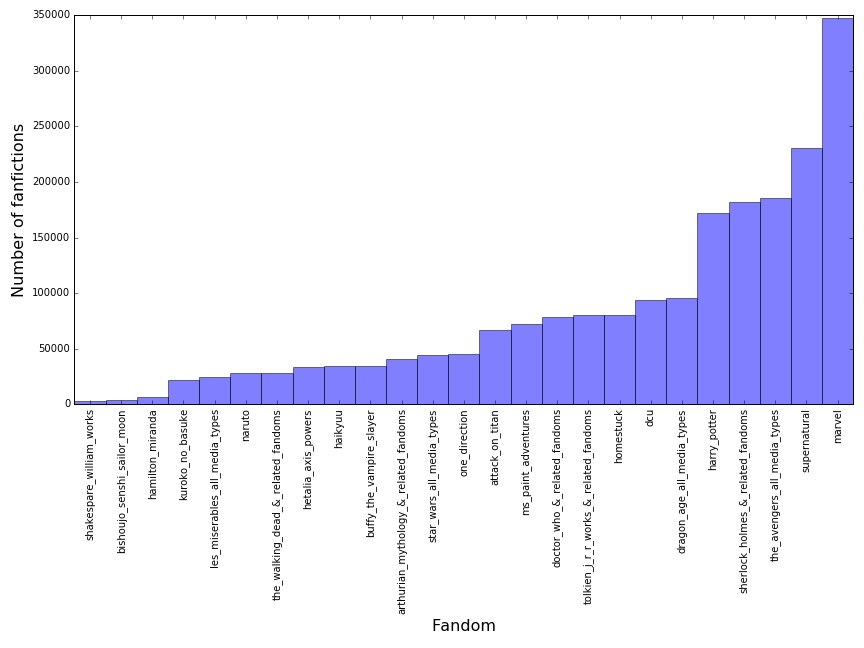
\includegraphics[width=\textwidth]{/fandom_size.pdf}
        \caption{Number of fanfictions in each fandom}
        \label{fig:fandom_size}
    \end{subfigure}
    ~ %add desired spacing between images, e. g. ~, \quad, \qquad, \hfill etc. 
      %(or a blank line to force the subfigure onto a new line)
    \begin{subfigure}[b]{0.8\textwidth}
        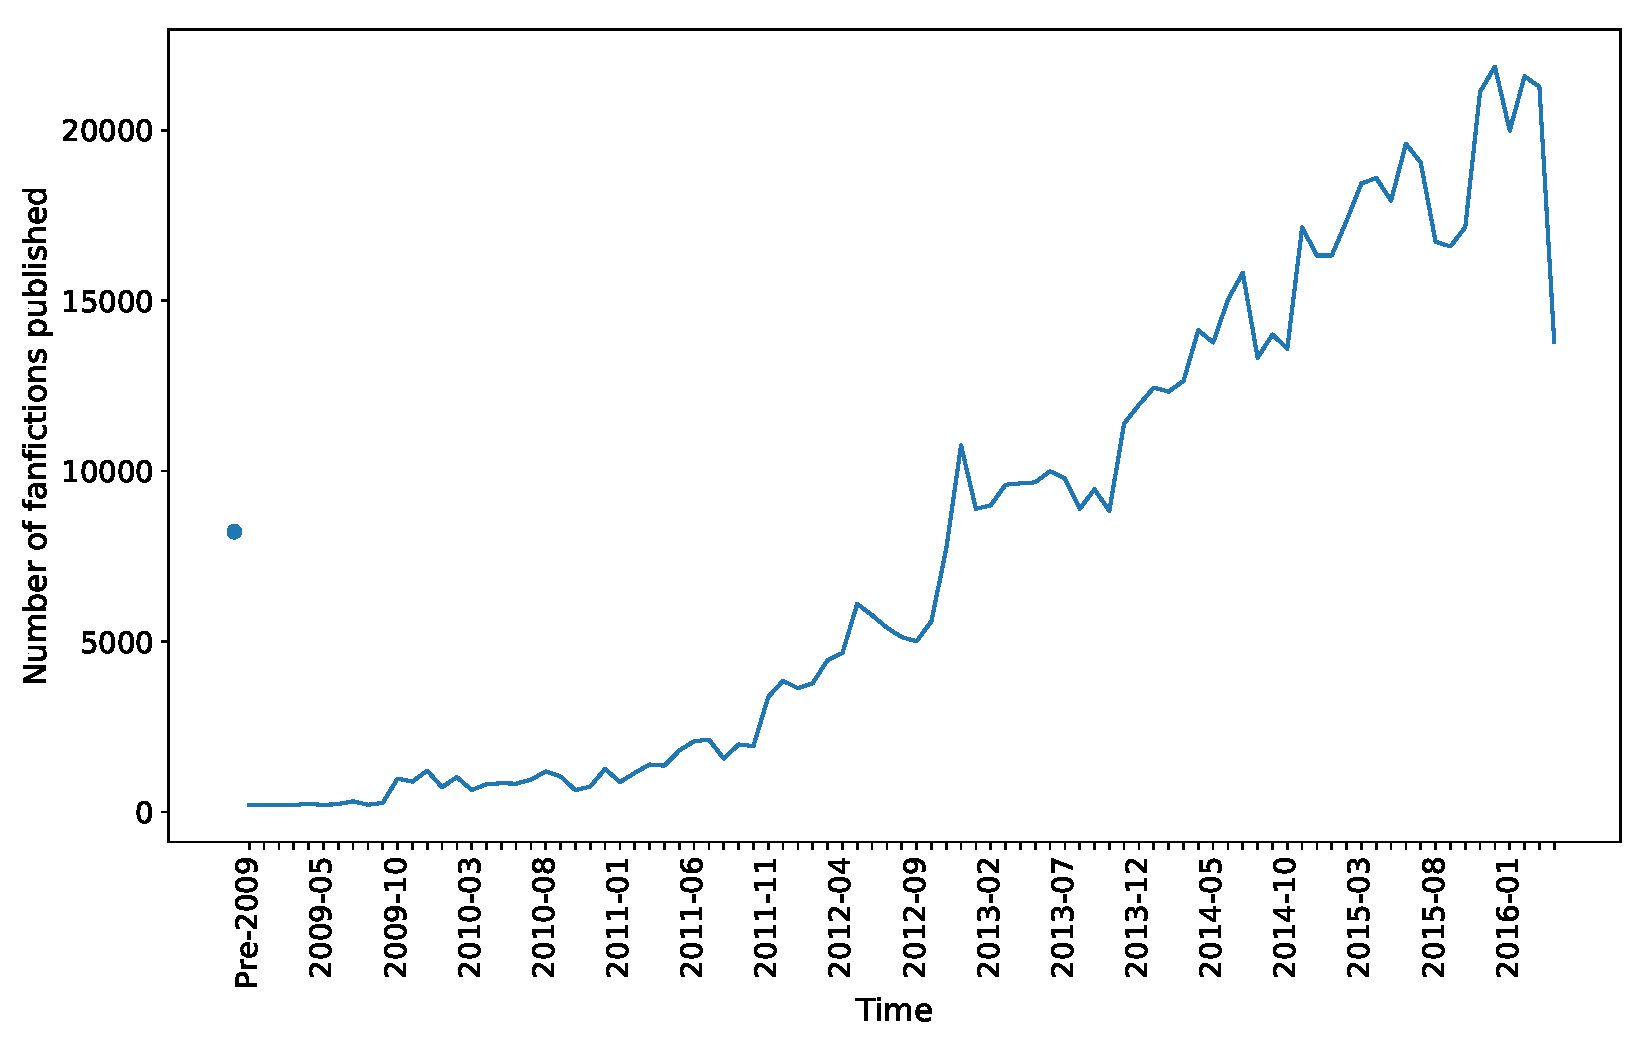
\includegraphics[width=\textwidth]{/fic_time_dist.pdf}
        \caption{Number of fanfictions published each month}
        \label{fig:fic_time_dist}
    \end{subfigure}
    \caption{The size of fandoms and the number of fanfictions published per month.}\label{fig:stats_size_time}
\end{figure}

Besides the fanfictions' texts, we also collected metadata including 14 fields. Some of them provide information about the fanfictions, while some can be used to evaluate the success of the fanfictions. Table \ref{tab:metadata} lists the names and descriptions of these fields. 


\begin{table}
\centering
\begin{tabular}[width=0.8\textwidth]{p{3cm}p{10cm}}
\toprule
\ Fields & Description \\ 
   \hline			
Title & Titles of the fanfictions.  \\
Fandoms & The fandom(s) that the fanfiction belongs to/ \\
Author & The author of the fanfiction.  \\
Publish Date & The date the fiction was published \\
Chapters & The number of chapters that a fanfiction have. \\
Archive Warnings & The warnings for sensitive elements in the fanfiction. \\
Category & The type of relationships in the fanfiction. \\
Rating & The rating of the fanfiction. \\
Relationship & The relationship(s) between characters in the fanfiction. \\
Age & The number of days between the last update of the fanfiction and time of the study. \\
\hline
Hits & The number of times a fanfiction is clicked on. \\
Bookmarks & The number of people who bookmarked the fanfiction.\\
Kudos & The number of ``like'' that the fanfiction receives. \\
Comments & The number of comments that a fanfiction receives.\\
\bottomrule
\end{tabular}
\caption{Metadata fields of the fanfictions.}
\label{tab:metadata}
\end{table}%

A fanfiction's success is most directly shown by its kudos, which is a direct expression that a reader likes the fiction. The hits is also an indicator of popularity. A reader may choose to bookmark a fanfiction to read later. This may depend on multiple motivations, such as the length of the fiction and the time when the reader browses the website. Moreover, we do not know if the reader returns to read the fiction later. The number of comments shows the engagement of readers with a fanfiction, and is  indirectly associated with popularity. Based on these considerations, we choose to use kudos as the primary indicators of success, and hits, comments and bookmarks as secondary indicators. The correlation between these indicators can be found in Figure \ref{fig:corr}. Figure \ref{fig:kudos_dist} shows the logged cumulative distribution of kudos and comments. Following long-tailed distributions, a small number of fictions receive the majority of kudos and comments, while most fictions receive little or none. 

While we are interested in how a fanfiction's novelty influences its success, there are many other factors at play. For example, some fandoms have large fan bases than others, resulting in a high average Kudos for the fanfictions in these fandoms. The popular authors' fame may influence how their works are received. Since AO3's user base has been increasing, we may expect newer fanfictions to receive more Kudos than older ones. Multi-chapter fanfictions are also likely to receive more Kudos than single-chapter ones. The archive warnings indicate that the fanfictions contain sensitive elements such as graphic violence or major character death, and may influence the readers' choice of whether to view them.  Other intrinsic features, such as the ratings of the fictions and the relationships in them may also influence the readers' preferences. In subsequent analysis, we use multiple methods to control for such influences.

\begin{figure}
    \centering
        \includegraphics[width=\textwidth]{/kudos_comments_hits_bookmarks_dist.pdf}
        \caption{Linear-log cumulative distribution of kudos, hits, bookmarks and comments. For multi-chapter fanfictions, we average these values over the number of chapters. A long-tail distribution is observed, where a small portion of fictions receive many kudos and comments, and most fictions receive view.}
        \label{fig:kudos_dist}
\end{figure}


\subsection*{Fanfictions' Novelty and Success}
Following the approaches by \cite{askin2017makes} and \cite{de2015game}, we evaluate a fanfiction's novelty by comparing it to other fanfictions previously published. Intuitively, if a fanfiction is close to the center of a feature space containing all past fictions, it is less novel; reversely, a peripheral position indicates higher novelty. 

We embed the fanfictions in the feature space using two methods. The first one is an vector space model as often used in information retrieval \cite{turney2010frequency}, where each fanfiction is represented as a vector, its entries being the term frequency-intersed document frequency (TFIDF) score of the unique words in the fiction. This allows us to identify the most representative terms in the documents, quantifying the term-level novelty. The feature space is created in a way that for each fanfiction, it contains all fanfictions published in the same fandom within the past 6 months before it was published. We then compute the center of the feature space as the average of all feature vectors. The \emph{term novelty} score of a fanfiction is defined as the cosine distance between its vector representation and the center:

\begin{equation}
n = 1-\frac{\sum_{i=1}^{n}{F_iC_i}}{\sqrt{\sum_{i=1}^{n}{C_i^2}}\sqrt{\sum_{i=1}^{n}{C_i^2}}}
\end{equation}

Where $F_i$ is the vector representation of a fanfiction and $C_i$ is the center of the vector space.

Alternatively, we also use the \emph{Latent Dirichlet Allocation} (LDA) \cite{blei2003latent} to model the topics of the fanficitions, quantifying novelty on the topic level. As a widely used topic modeling method, LDA models a fiction as a probabilistic distribution over a set of topics. Similar as in the previous method, we construct for each fanfiction a feature space consisting of the topic distributions of the fanfictions published before it, and define the \emph{topic novelty} score as the cosine distance between the fanfiction's topic distribution and the center. 

Figure \ref{fig:tfidf_lda_kudos} plots the relationship between the fanfictions' novelty and the kudos they receive, aggregating all fandoms. Since the fandoms differ in reader base, we compute the z-score for each value of kudos based on the average number of kudos per fanfiction in its fandom. We observe that as the term novelty score increases from 0  to 1, the z-score of Kudos steadily decrease from 0.1 to -0.1 in the vector space model, and from more than 0.1 to -0.03 as the topic novelty increases in the LDA model. In both cases, the less novel fanfictions receive more than average kudos, and the highly novel fanfictions receive less than average. Similar patterns can be observed between novelty and hits, comments and bookmarks (See future supplementary figures).

\begin{figure}
    \centering
          \includegraphics[width=\textwidth]{/novelty_tfidf_lda.pdf}
        \caption{The relationship between novelty and kudos. Left: term novelty. Right: topic novelty. The x-axes are the novelty scores, and the y-axes are the corresponding average of the z-score of kudos in bins with bin size = 0.1. The confidence intervals are generated with bootstrap resampling. }
        \label{fig:tfidf_lda_kudos}
\end{figure}


We perform a regression analysis to further explore this relationship. Instead of using the z-scores as in previous analysis, here we use the logged values of kudos, hits, comments and bookmarks as outcome variables. The term novelty and topic novelty scores are used as predictor variables. A few other control variables are added to account for the influence of other factors on the reception of fanfictions. First, the number of chapters that a fanfiction has is included, considering that since AO3 displays the newest post on the top, multi-chapter fictions have more chances of exposure. Secondly, categorical variables are created to capture the effects of the fandoms, archive warnings, authors, categories, ratings and the relationships on a fanfiction's success. Finally, we include the age of each fanfiction as a numerical variable. The correlations between the numerical variables are shown in Figure \ref{fig:corr}. As no strong correlation exists between the predictor variables, we do not need to consider this effect.

\begin{figure}
    \centering
          \includegraphics[width=0.8\textwidth]{/variables_corr.pdf}
        \caption{Correlations between the predictor and outcome variables. Strong collinearity exists between the outcome variables, but not the predictor variables. }
        \label{fig:corr}
\end{figure}

A pooled OLS is run for each outcome variable, multiple-regressing on the predictor variables. The coefficient estimates of the multiple regression are summarized in Table \ref{tab:regression}. They further support our previous observation that higher novelty contributes to a fanfiction's receiving less kudos, hits and bookmarks. A much lower r-squared value for comments suggests that the model does not account for comments very well. As the reception of a fanfiction is shaped by many factors including possible kinds of noise, we consider the signals found with this model to be a strong indicator of the negative contribution of novelty to successful fanfictions.

 \begin{table}
\centering
\begin{tabular}[width=0.8\textwidth]{p{3cm}p{3cm}p{3cm}p{3cm}p{3cm}}
\toprule
\ Outcome variable: & Kudos & Hits & Comments & Bookmarks \\ 
   \hline			
Term novelty & --0.6080***&  -0.4366***  & -0.1043*** & -0.2767*** \\
& (0.008) & ( 0.007) & (0.008) & (0.010)\\
Topic novelty & --2.5085*** & -2.0841*** & -0.8142*** & -1.9733*** \\
& (0.047) & (0.043) &  (0.044 ) & (0.057)\\
Fandom & 0.0061*** & 0.0097*** & 0.0064*** & -0.0012*** \\
& (0.000) & (0.000) & (0.000) & (0.000)\\
Chapters & -0.0063***& -0.0039*** & 0.0015***& -0.0059*** \\
& (5.33e-05) & (4.88e-05) & (4.39e-05) & ( 5.67e-05) \\
Archive warnings & 0.0011 & 0.0006*** & 0.000***& 0.0011 ***(\\
& (4.26e-05) & (3.9e-05) & ( 3.99e-05 ) & 5.14e-05)\\
Author & 3.932e-06*** & 2.883e-06***& 7.349e-07*** & 1.815e-06***\\
& (9.96e-08) & (9.12e-08) & (9.41e-08) & (1.21e-07)\\
Category & 0.0023***& 0.0019***& 0.0006*** & 0.0018***\\
& (2.51e-05)  & (2.3e-05)  & (2.45e-05) & (3.16e-05)\\ 
Rating & -0.0720*** & -0.0791***& -0.0360*** & -0.0341***\\
& (0.001) & (0.001) & ( 0.001) & (0.001) \\
Relationship & 1.833e-05*** & 2.275e-05***&  2.765e-06*** & 4.863e-06***\\
& (2.85e-07) & (2.61e-07) & (2.78e-07) & (3.59e-07) \\
History & -0.0002***& 0.0002*** & -9.132e-05 ***& 0.0003***\\
& (4.87e-06) & (4.46e-06) & (5.39e-06) & (6.95e-06)\\
\hline 
Observations & 354978 & 354978 & 354978 & 354978 \\
R-squared & 0.111 & 0.099 & 0.028 & 0.099\\
\bottomrule
\end{tabular}
 \begin{tablenotes}
      \small
      \item Standard errors are in parentheses.
      \item ***p < 0.001.
       \end{tablenotes}
\caption{OLS results}
\label{tab:regression}
\end{table}%

\section*{Discussion}
We have developed a way to quantify the novelty of a fanfiction by locating it in a feature space, comparing it to other fanfictions in the same community. This also allow us to measure novelty of a piece of creative writing on different scales, including words and topics. Although we choose to focus on fanfictions, our method can be easily extended to other types of creative writings.

Our findings show that fanfictions with high novelty receive less positive feedbacks from readers, and the successful fanfictions are those with low novelty. This pattern diverges from many existing researches, which find reversed U-shapes with the peak of success being creative works with a moderate amount of novelty. A possible explanation may be the nature of fan works -- because fans desire to see familiar characters and stories, it is reasonable for them to prefer fanfictions that are familiar to them. A similar reasoning may explain people's desire to consume familiar culture products, such as listening to songs that they have listened to before \cite{thompson2014shazam}, and may justify the abundance of sequel and spin-off works in today's pop culture scene. 

\section*{Methods}

\subsection*{Data collection}
A Python script was used to obtain data from AO3 (http://archiveofourown.org/) as csv files in March 2016. We filtered the data based on the language and length of the fanfictions, and removed entries with missing data. For more details, see Results.


\subsection*{Modeling fanfictions}
The Python library scikit-learn was used to create the vector space models. Another library Gensim is used to fit LDA topic models on our data. We set the number of topics to 100 and use default values for other parameters. 



\bibliographystyle{acm}
\bibliography{main}

% https://academic.oup.com/chemse/article/24/2/191/312277 familarity & hedonic value of odors
% http://rsos.royalsocietypublishing.org/content/4/7/170433  Significance and popularity in music production

    
\end{document} 



%The authors and readers' passion about fanfictions alludes to a balance between novelty and familiarity: they desire to see familiar characters and elements, but in novel stories. By analyzing people's perception of fanfictions, we may gain a better understanding of this balance. 

%Researches are only starting towards a quantitative definition of novelty. Many have employed a network approach, defining a creative work's novelty by looking at how they reference previous works \cite{elgammal2015quantifying}\cite{wang2013quantifying}\cite{2017arXiv170704239I}. In some cases, tags of a work can be used to evaluate its novelty\cite{sreenivasan2013quantitative}. 

%While the text of fanfictions directly capture their contents, the tags generated by authors (see Methods) provides a summary of the fictions. Authors often use tags to describe the genre and plot of their fictions, for example, ``Angst'' or ``Alternative Universe''. Although a user is free to use any tag, when she starts to enter a tag, the website will prompt with tag suggestions, avoiding multiple synonyms. The tag set of a fiction provides an abstraction of its content. Besides the language modeling approach, we also ran a separate analysis on the tag set.

%Story telling is one of human beings' basic needs and abilities\cite{gottschall2012storytelling}. Despite having endless forms, most stories can be considered as variations of one of the basic archetypes. In mythology studies, Campbell deduced a fundamental structure, \emph{the hero's journey}, from all major myths around the world \cite{campbell2008hero}. Levi-Strauss broke down different versions of a myth to identify common mythemes \cite{levi1955structural}. In oral legends and tales, many stories had a certain origin and developed into different versions through time and interaction between creators. Myths and folktales in oral traditions of civilizations around the world often follow this pattern, for example, the tale of the \emph{Little Red Riding Hood} originated approximately in the 10th century, and has developed multiple variations\cite{littlered}. Some elements of the legend \emph{Mahabharata} can be traced back to the Vedic period (15--6 century B.C.) as oral tales told by bards, and was textualized into many versions\cite{van2011mahabharata}.

%Thomas \cite{thomas2011fanfiction} summarizes the study of fanfictions into several main stages: Earliest researches characterized the fanfiction writers as "rebels" against the powerful authority of the original work. Later researches attempted to generate a deeper understanding to this simplified view, and started responding to the new media forms that facilitated fan activities and interactions. Some recent studies shifted their emphasis to the contributions of fans to contemporary culture. 

% Similar to other creative works, fanfictions are constantly under selection and evaluation from their readers. %The most successful fanfictions in the market have been published and even adapted into other media forms, accepted by the main stream (for example, \emph{Fifty Shades of Grey} was originally a fanfiction of \emph{Twilight}), while the majority of them remain mostly unknown.


%The length distribution of the fanfictions is presented in Figure \ref{fig:length_dist} . Since many fictions have multiple chapters, we consider length as the average number of words in each chapter. A great variation of average length can be observed. The variation of length in documents can have a significant effect on the distance between documents, biasing towards shorter distance between longer documents. A similar issue has been noticed in vector space models very early on \cite{singhal2017pivoted}, where many normalization methods have been proposed to correct it. Instead of applying a normalization, in our analysis, we sample a fixed length (1,000 words) from each document. 

%In Figure \ref{fig:tag_set_len}, we observe the tag set length of the fictions. The majority of fictions has under 20 tags, with a few having as many as 150 tags. Because the users have the liberty to create any tag, many of the tags will not be reused. To reduce the influence of infrequent tags, we therefore discard the tags that appear only once.
